\justify
\only<1>{This is description 1}
\only<2>{This is description 2}
\only<3>{This is description 3}
\end{overlayarea}
\column{0.5\textwidth}
\begin{overlayarea}{\textwidth}{\textheight}
\begin{figure}
\centering
\only<1>{\includegraphics[scale=0.5]{1}}
\only<2>{\includegraphics[scale=0.5]{2}}
\only<3>{\includegraphics[scale=0.5]{3}}
\end{figure}
\end{overlayarea}
\end{columns}
\end{minipage}
\begin{minipage}[t][0.4\textheight][t]{\textwidth}
\begin{overlayarea}{\textwidth}{\textheight}
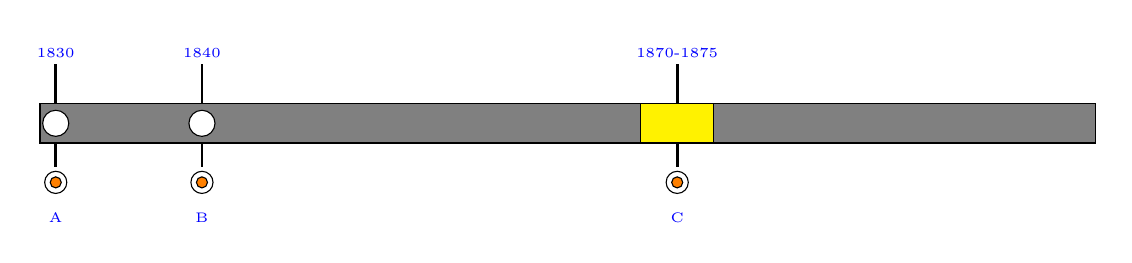
\begin{tikzpicture}[datemarker/.style={circle, draw=black,fill=white},textlabel/.style={anchor=center,text height=1.7ex,text depth=.25ex}]
\tikzset{every node/.style={font=\tiny, color=blue}}\draw[fill=gray](-0.2,0) rectangle (13.2,0.5) node[white, below]{};
\onslide<1->{\node at (0.0, 0.25) [datemarker] {};}
\onslide<1->{\draw [line width=1pt] (0.0, 0.5) to (0.0, 1.0);}
\onslide<1->{\draw (0.0, 1.2) node [textlabel]{1830};}
\onslide<1->{\draw [fill=orange](0.0, -0.5) circle (2pt){};}
\onslide<1->{\draw(0.0, -0.5) circle (4pt){};}
\onslide<1->{\draw [line width=1pt] (0.0, 0) to (0.0, -0.3);}
\onslide<1->{\draw (0.0,-0.9) node [textlabel] {A
};}
\onslide<2->{\node at (1.85714285714, 0.25) [datemarker] {};}
\onslide<2->{\draw [line width=1pt] (1.85714285714, 0.5) to (1.85714285714, 1.0);}
\onslide<2->{\draw (1.85714285714, 1.2) node [textlabel]{1840};}
\onslide<2->{\draw [fill=orange](1.85714285714, -0.5) circle (2pt){};}
\onslide<2->{\draw(1.85714285714, -0.5) circle (4pt){};}
\onslide<2->{\draw [line width=1pt] (1.85714285714, 0) to (1.85714285714, -0.3);}
\onslide<2->{\draw (1.85714285714,-0.9) node [textlabel] {B
};}
\onslide<3->{\draw[fill=yellow](7.42857142857,0) rectangle (8.35714285714, 0.5){};}
\onslide<3->{\draw [line width=1pt] (7.89285714286, 0.5) to (7.89285714286, 1.0);}
\onslide<3->{\draw (7.89285714286, 1.2) node [textlabel]{1870-1875};}
\onslide<3->{\draw [fill=orange](7.89285714286, -0.5) circle (2pt){};}
\onslide<3->{\draw(7.89285714286, -0.5) circle (4pt){};}
\onslide<3->{\draw [line width=1pt] (7.89285714286, 0) to (7.89285714286, -0.3);}
\onslide<3->{\draw (7.89285714286,-0.9) node [textlabel] {C};}
\end{tikzpicture}
\end{overlayarea}
\end{minipage}
\end{frame}
\end{document}
